\subsection*{Progress beyond state of the art}

\begin{longtable}{|p{0.2\textwidth}|p{0.75\textwidth}|}
\hline
{\bf Networking activities}
&
In order to foster a culture of cooperation between scientific
communities that are often too focused on their problems, this project
will develop several networking activities.\\
&
\hspace{0.4cm}
The initial phase of the project, the development of a common
infrastructure, will be the first step in the networking activities of
the twenty-eight project partners. Thereafter, collaborations between
partners will grow, allowing them to better use the Logipedia
infrastructure to meet their needs as well as those of users outside
the project. This effort will develop the formal proof community in
the countries where it is still in an early stage of development.  To
structure this growth, several user groups will be created: 
in industry, in academia, in education, and in publishing.\\
&
\hspace{0.4cm}
The industrial partners of the project
and yhe club of industrial users 
will strengthen a culture of cooperation between scientific
researchers and engineers in academia and in industry. Currently this
cooperation is too often point-to-point (for instance, an enterprise uses
one system and develops links to a group of academic researchers
developing this system). But we need to develop a more comprehensive
culture of cooperation, around common languages and a common research
infrastructure.\\
&
\hspace{0.4cm} Our action in this direction is twofold. First, some
enterprises that already have a strong commitment in formal methods
(Clearsy, CEA, MED-EL, etc.) are included in the project as
partners. Other enterprises that could not be part of the project
because of its limited size, or that have a less developed culture in
formal methods, are members of the club of industrial users. Among
other goals, this club participates to develop a culture of
technology watch in formal methods in industry, which is a stepping
stone for developing a strong industrial awareness in safety and
security in European industry. This club is also only in its initial
phases, but we are confident that the initial members of this club
will be followed by others.\\ 
&
\hspace{0.4cm}
The club of academic users
we will develop a similar culture of technology watch for
researchers who are outside formal methods.  
It gathers colleagues from our community that could not participate to
this project, as well as colleagues from outside the formal methods
community, in particular mathematicians who are understanding
the long term impact formal proofs will have on mathematics.\\
&
\hspace{0.4cm}
The club of users in education
will also to develop a similar culture of
technology watch for teachers, including high school teachers who are
investigating how a library of formal proofs can be used with younger
students. Here we do not advocate teaching formal proofs to pre-schoolers, but
we aim at fostering a culture of rigor in high-school mathematical
thinking, by having rigorous statements of theorems in high-school
textbooks (including all the corner cases that are often omitted), as
well as a clear structure of how each proof of a theorem relies on
other theorems. This improved rigor is useful for both the students
who will study sciences at University and to those who will not. In
particular, in this way we want to modestly contribute to the renewal
of the logical thinking culture, which is of prime importance in our
``post-truth era''.\\
&
\hspace{0.4cm}
We also believe that an early exposition to formal statements and / or
formal proofs may contribute to compensate the gender disparity
in our research community. Here also, we must remain modest, as
achieving a decent gender-balance will require more than a single
action, but is is obviously much more effective to try to promote
contemporary scientific ideas, and encourage scientific carriers, to
women at the high school level rather that at the university level,
because at the university level there are already too few women in
our auditoriums.\\
&
\hspace{0.4cm}
The club of users in publishing 
will develop networking activities with publishers
(Elsevier, Springer, etc. but also, ArXiv, HAL, Wikipedia, etc.)~
such that formal proofs mentioned in research papers and in
other encyclopedia can be permanently made accessible, in Logipedia, 
while they currently often are just made accessible
on the web page of the authors.\\
&
\hspace{0.4cm}
These four clubs of users: industrial users, academic users, users in 
education, and users in publishing, together with the partners of the 
project, will also
prepare a larger community that will develop Logipedia beyond the end
of the project, in order to achieve our ultimate goal of making
Logipedia contain all the formal proofs then developed in twenty
years.\\
&
\begin{center}
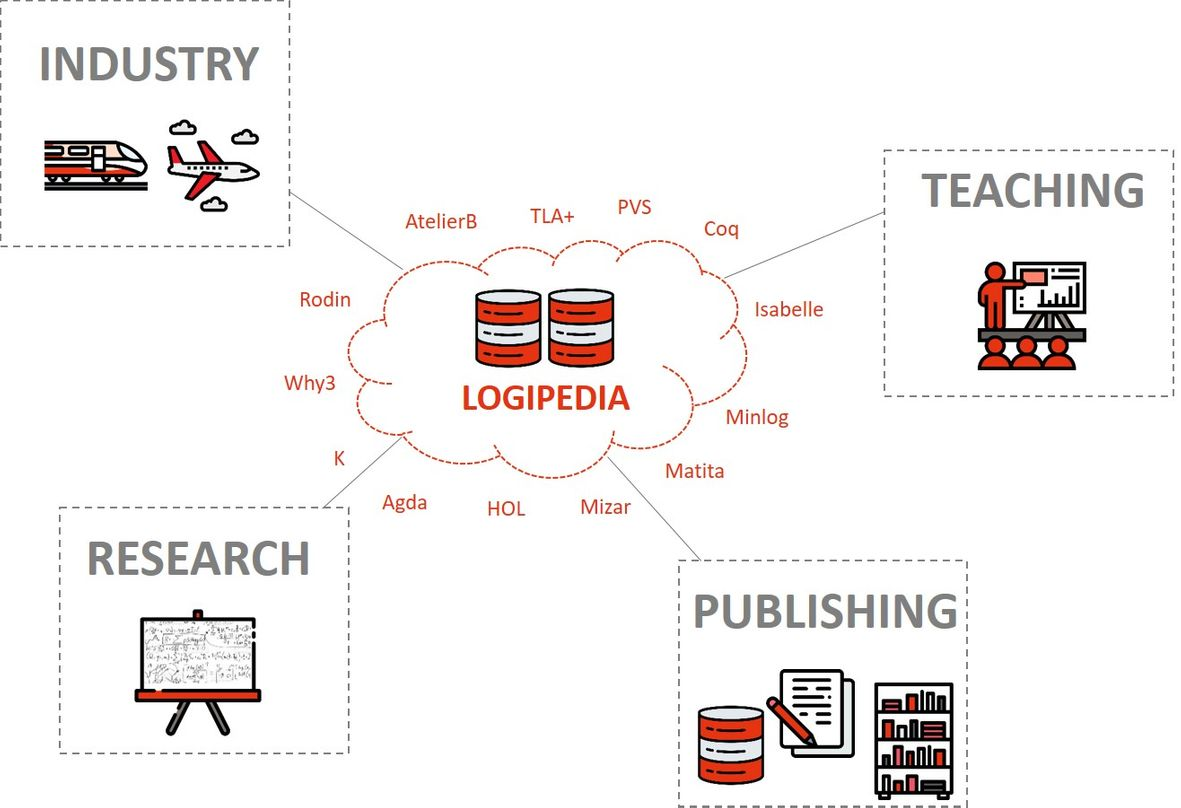
\includegraphics[width=12cm]{img/Schema-reduced}
\end{center}\\
&
\hspace{0.4cm}
Finally, this project also prepares the exploitation of Logipedia
beyond the duration of the project.\\
&
\hspace{0.4cm}
Of course, we plan to organize the usual networking activities,
such as a yearly conference with associated workshops on applications
in industry, research, education and publishing, a general assembly
where the research directions can be discussed collectively. We also plan to organize
summer schools, especially at the beginning of the project in order to
train the new participants (doctoral students, post-docs, etc.) to the
technology developed in Dedukti and Logipedia
(see Section Dissemination and Communication.)\\
&
\hspace{0.4cm}
So developing jointly such an infrastructure will not only reconfigure
the research community on formal methods, but also the industrial
community on formal methods, and will build bridges with the communities
of education and of publishing.\\
\hline
{\bf Trans-national access and virtual access}
&
Logipedia will be accessible online. It will therefore be accessible
at no cost, and without identification, from every country in Europe
and beyond, just like, for instance, Wikipedia is.\\
&
\hspace{0.4cm} The licence chosen for the Logipedia proofs does not
need to be the same for all proofs, because some proofs already have a
licence before being imported in Logipedia and, in some cases, this
licence must be preserved.  Yet, in general we will favor a creative
common licence and in particular cc-by.  Such a licence allows a free
access, a findable, accessible, interoperable, and reusable data
management. It will contribute to the development of the Open data /
Open science / Open innovation philosophy and be in line with European
policies encouraging open science.
\\
&
\hspace{0.4cm} Being a central infrastructure, Logipedia will
contribute to strengthen the links within the European research area,
that it too scattered: for instance, currently, researchers and
engineers often use a system developed in their own country (only a
few systems having an international community of users), and the
libraries of formal proofs specific to this system.
\\
&
\hspace{0.4cm}
As explained above, our effort on access goes beyond providing a
trans-national and virtual access, as accessibility depends also on
developing an ergonomic web interface, a package distribution system,
a search engine, and an ontology of mathematical concepts. The public
targeted by these interfaces also has to be taken into account, a
secondary school student looking for a theorem in geometry needs a
different interface from a engineer looking for the correctness proof
of an algorithm.\\
\hline
{\bf Joint research activities}
&
The project includes joint research activities that would not be possible 
without this project of co-building an infrastructure.
\\
&
\hspace{0.4cm} Logipedia will allow joint research projects between
the users of this infrastructure that will be able to develop new
proofs together using different systems.\\
&
\hspace{0.4cm}
Then, Logipedia raises new research
problems. Some of them have already been solved in the past and
must be implemented jointly. Others are newer.\\
&
\hspace{0.4cm}
Using a common infrastructure requires
to describe the theories implemented in the different systems in a
common logical framework. We have already discussed how the expression
of geometry, arithmetic, and set theory in predicate logic has
enabled a renewal of logic at the end of the 1920's, allowing all
the logicians to speak the same language. Here we can expect a similar
renewal, fostering new joint research through the sharing, not
only of a common infrastructure, but also of a common language.\\
&
\hspace{0.4cm}
The development of a common encyclopedia, such as Logipedia, also
raises completely new problems such as automatic concept alignment,
structuring a large body of knowledge, or the development of
interfaces. These problems will trigger new cooperation between the
partners of the project and beyond.\\
\hline
\end{longtable}

\subsection*{Innovation potential}

Formal methods are at a turning point. Several academic and
industrial successes have proved the readiness of the technology,
in particular in critical systems where it has helped in
dramatically improving the quality of the systems. But this
technology takes too much time to be adopted in a broader context.

Limiting factors, probably the main ones, are the redundancy of the
efforts to develop proof systems, the lack of a common theory or at
least a common language to express the various theories, the lack of
common benchmarks, and the lack of standards for these systems.

For industry, at least three key aspects slow down the adoption of
formal methods.

First, reusing a proof produced with a particular tool in another, 
when it is even possible, can only be done at a high cost.
Logipedia will help reducing this cost by unifying tools
around a common format, enabling the possibility to share proofs
between tools. In the uncommon case where a proof relies on a theory
which is not compatible with the target tool, it will be easier to
understand why and determine whether adapting it is manageable.
Furthermore, as an infrastucture, Logipedia will help users
in finding existing proofs of properties, making their verification
process faster.

Second, checking a proof must remain possible over time. Today, it
requires either to maintain proofs along new versions of the tools,
which can represent a significant maintenance cost, or to archive
them together with a version of the tool used to produce it. In this
situation, Logipedia will help on two aspects. First, the
common format will guarantee that proofs can be checked by any tool
implementing it, thus reducing proof maintenance cost. Second, by
providing a common proof database, general interest proofs can be
stored and maintained in the infrastructure, allowing industrial users
to focus their resources for their specific needs only.

Finally, a proof or verification tool can be mistrusted. For example,
in a certification context, the use of a particular tool for the
verification of the candidate system must be approved. If the
certification body is not familiar with the tool, producing a
justification for it can represent a significant amount of time. For a
new tool, adoption is even slower, as not only certification bodies
but also potential users could question its soundness despite the
potential advantages it could provide. The common, co-built, format
offered by Logipedia will provide an answer to this lack of trust. It
will help the certification bodies, as they will not have to learn
about a new tool for each new certification process, as any tool
implementing the format will be suitable for them to check the
proof. Thus they only have to trust one. Consequently, it will also
help industrial users, as justifying the use of a particular tool will
be easier as long as they can provide a proof in the right format. And
finally, it will encourage the development of new tools, as potential
users will not have to trust these tools directly, but only the proofs
that they provide, which can be checked easily.

This project to integrate the scientific and technological effort
around formal proofs in Europe is thus a way to foster the
development of formal methods in industry, as the economic spinoffs
from the project will benefit the European industry, mainly by reducing
the cost of this technology. Let us mention how Logipedia is viewed by 
some of the members of our club of industrial users. 

{\bf Alstom} is a major rolling stock and railways signalling systems
supplier with more than 35,000 employees all over the world. It
provides its customers in more than 25 countries with safety-critical
systems that prevent hazardous situations for passengers, staff and
equipment while ensuring fluent and cost-effective operation.

For more than 30 years, Alstom has been developing or verifying with
formal methods some of its safety-critical signalling systems. He is
therefore an intensive end-user of proof systems (Atelier B, S3, Why3,
Isabelle) and highly concerned and interested in all projects that can
improve the quality and efficiency of its proof activity. This is the
reason why Alstom is highly interested in the Logipedia project and
wants to be an active member of its industrial user group.

{\bf Arm} is the world's largest provider of semiconductor IP and
is the architecture of choice for more than 90\% of the smart
electronic products being designed today: Arm designs have found their
way into more than 20,000,000,000 devices in 2018, for instance.
Increasingly, the Arm architecture is also being deployed in
supercomputers and servers, with Amazon’s AWS recently announcing its
Graviton line of Arm-based high-performance servers.

As well as the 32- and 64-bit CPU cores, their hardware products
extend to GPUs, DSP cores, cell libraries, memory compilers and system
components. Arm also produces a wide array of software products, many
of which are extremely security- sensitive: low-level firmware,
privileged security monitors, operating system kernel patches,
cryptography libraries, and transport layer security protocol
implementations are all developed and actively maintained by Arm
engineers on behalf of their wider ecosystem, for example. Arm
engineers also play an active role in developing and standardising
novel cryptographic protocols and ciphers through various
international bodies.

Given the ubiquity of the Arm architecture, Arm has an
obvious interest in ensuring that various functional and security
properties hold, and also that its microprocessor designs are indeed
correct instantiations of this architecture. As a result,
semi-automated formal techniques have long been used within the
company to ensure the correctness of our architecture and of our
microprocessor designs.

Whilst many of their verification flows have been built around
commercial tools that they license ``off-the-shelf'', they also
developed their own formal tools using SAT and SMT technology, and
many of these tools are in active use by our product engineering
groups. Moreover, we are increasingly experimenting with:

\begin{compactitem}
\item The deployment of formal techniques as an enhanced bug-finding
  mechanism for especially sensitive software products, using
  bounded-model checking technology and SMT-based pre/postcondition
  checking, using tools such as the C-bounded model checker (CBMC) and
  Frama-C.
\item Model checking novel locking mechanisms for highly concurrent
  code, to spot potential deadlocks, using the TLA model checker.
\item Formally documenting and semi-automatically finding security
  flaws in cryptographic protocols using dedicated model checking
  tools, such as Tamarin.
\end{compactitem}

However, often they would like to establish deeper properties of the
architecture and of their software implementations than can reasonably
be obtained using the semi-automated formal approaches described
above. For this reason, they have ongoing experiments with the use of
interactive theorem proving, using both Coq and Isabelle/HOL, two
popular tools that have shown promise in academia on a range of
software and hardware verification projects.

From Arm’s perspective, ideally there would be some way of
transferring definitions and proofs between some of these tools so
that we can maximise reuse, avoid wasted engineering effort, and also
potentially share the models that we develop and associated proofs
with the many communities surrounding these tools for use in academic
projects. Unfortunately, to our knowledge no robust mechanism exists
at present that can achieve this and therefore writing a formal model
in Coq almost certainly precludes the Isabelle/HOL community from
using that model without significant duplication of engineering
effort, for example, and vice versa.

In light of the above, Arm is especially excited by the Logipedia
project which aims to facilitate the sharing of definitions and proofs
between many different interactive theorem proving systems,
considering the problem a long-standing issue that is holding back
commercial adoption of interactive theorem proving technology.
Moreover, Arm wishes to keep track of the project as it progresses,
and potentially provide insight from their industrial use of formal
methods technology. For this reason, they are committing to joining
the Logipedia industrial users club.

{\bf Edukera} has developed an online educational application to teach
mathematics which relies on the use of the formal proof assistant Coq
(developed by Inria).

One of the key features is the ergonomic design of the numerical
mathematical paper which allows students to build the proof with point
and click interactions. This numerical paper has been developed and
improved over several years of experiment with students' and teachers'
feedback. So much so that the Edukera application is currently the
most advanced user interface to do mathematical proofs in education.

Since its commercial launch in 2016, the Edukera application has been
successfully used in many universities by 8,000 students to solve
250,000 exercises.

Over the years Edukera has experienced an increasing need for formal
methods in education. This is due to the emergence of new industrial
activities (cryptocurrency and the verification of smart contracts,
software dependant autonomous vehicles, \ldots). This is why Edukera
considers the existence of a solid open-source education-dedicated
interface for formal proofs, to be critical to the upcoming industrial
ecosystem.

However, several issues in the design of the current Edukera
application prevent a larger user base and need to be solved:
developers in formal methods need to create their own theories and
teachers must be able to develop their exercises; plus the core
Edukera solution should be open-sourced for anyone to use, fix and
improve when necessary.

The use of Logipedia as the mathematical foundation of the Edukera
application can solve these critical issues: indeed Logipedia
federates a large scientific community around a unique language, and a
large developer community around a unique open-source mathematical
framework, which is beyond the financial means and traction of the
Edukera company on its own.

Students may already access the Edukera application and
exercises. Hence the existence of an open-source version of the
Edukera application will not affect the business model which is based
on the billing of class administration features (activity reports,
homework schedule, connection to the LMS, \ldots).

For these reasons, Edukera is willing to join the club of industrial
users of Logipedia.

{\bf Facebook} AI Research (FAIR) is the fundamental research lab in
Artificial Intelligence of Facebook. Its largest research center in
Europe is in Paris and has been employing over 70 people, mixing
researchers, engineers and students for over four years now. FAIR is
recognized as one of the top leading AI labs in the world and is proud
of doing fundamental research. FAIR actively engages with the research
community through publications, open source software, participation in
technical conferences and workshops, and collaborations with
colleagues in academia. FAIR has hundreds of academic partners across
the world, such as Inria.

FAIR Paris has a team working on deep learning for theorem proving, a
long-term effort in academic research. It uses existing formal proofs
as its learning datasets and is interested by the Logipedia project as
a possible source of training data. FAIR Paris also has a strong
interest in automatic language translation and would be keen to apply
this to formal proof languages.

Facebook is therefore willing to join the club of industrial users
that the Logipedia project wants to create.

{\bf IBM}'s Thomas J. Watson Research Center serves as the
headquarters of IBM Research -- one of the largest industrial research
organizations in the world -- with 12 labs on 6 continents. Scientists
at T. J. Watson, and at IBM around the globe, are pioneering
scientific breakthroughs across today's most promising and disruptive
technologies including the future of artifial intelligence, blockchain
and quantum computing. In all of these areas, formal proofs can bring
benefits ranging from reducing bugs to having a deep and fundamental
understanding of the studied objects.

The Logipedia project is of strong interest for IBM
Research. Developing proofs requires a huge effort. Being able to
reuse formally proved properties could reduce the development time and
thus allows to tackle larger problems. Moreover, each proof assistant
requires its own expertise. The ability to reuse proofs coming from
any system in the proof assistant of our choice is therefore a great
benefit.

That is why IBM Research would like to join the club of industrial
users of Logipedia. IBM Research would also be happy to contribute to
the project with Q*cert, a data base query compiler developed in Coq,
and could then be translated to other proof assistants thanks to
Dedukti and the tools developed around Dedukti.

{\bf Mitsubishi Electric} is one of the world's leading names in the
manufacture and sales of electrical and electronic products and
systems used in a broad range of fields and applications, in
particular energy and electric systems, industrial automation,
information and communication systems, electronic devices, and home
appliances. One of Mitsubishi Electric's objectives consist in
creating new value through innovation and promoting R\&D that persues
sustainable growth. For that purpose, Mitsubishi Electric devotes 5\%
of its revenue to its research and development budget, contributing to
realizing Society 5.0 and achieving the goals of the United Nation's
sustainable development goals.

Mitsubishi Electric R\&D Centre Europe believes that for achieving
those sustainable goals, one of the key factors is the confidence one
can have in software, that drives people and more people's life,
industry, etc. That's why it has studied for more than ten years
different formal methods theories and tools that can help designing,
specifying, implementing and maintaining software. Its objectives is
to fill the gap between state of the art academic work and industrial
objectives and processes, to bring the power of formal methods to
regular engineers. Among those formal methods, formal proofs allow to
reach the highest level of confidence in software, but they are also
the hardest to manipulate for non-specialists. Mitsubishi Electric
R\&D Centre Europe sees the Logipedia project as an important
milestone for widening access to formal proofs, and helping their
dissemination in industry for two reasons. First, by giving to an
encyclopedia of off-the-shelf and ready-to-use formal proofs, avoiding
to prove many times the same properties. Second, by also strengthening
the European formal proofs community and helping them to provide a
kind of unified interface to industry problems.

For those reasons, Mitsubishi Electric R\&D Centre Europe strongly
supports the Logipedia project proposal and intents to participate to
its club of industrial users.

{\bf Nomadic Labs} is a R\&D company that contributes to the
development of the Tezos protocol. It gathers experts in formal
methods, distributed systems, and programming language theory and
practice. It puts a particular emphasis on formal verification, and
uses and develops related tools, applying them to the Tezos codebase,
algorithms, and smart contracts. Nomadic Labs uses mostly the Coq and
F* proof assistants, and supports the development of Coq and other
tools dedicated to formal verification through its partnerships with
premier research institutes.

The Logipedia project aims to create a library of formal proofs in a
common pivot language called Dedukti. The existence of such a
populated library, and the possibility of bringing proofs from one
proof system to another one, will favor the general use of formal
verification by avoiding the duplication of efforts, and encouraging
proof reuse.

Nomadic Labs is of course very interested by such a project and is
willing to be a member of the club of its industrial users.

{\bf Onera} has research activities in the development and application
of formal methods for critical systems and software for aerospace
applications. We believe formal techniques are useful for risk
analyses, safety and security assessment of critical systems,
development and verification of critical software. We apply formal
techniques for aerospace applications (aircrafts, UAVs, robotics). We
have also been part of the international group that defined DO-333
(formal methods technical supplement to DO-178, software certification
standard for aeronautics).

Onera agrees on the significance of the problems addressed by the
Logipedia infrastructure, and has a serious interest in the approach
of the Logipedia project to tackle these problems.

Onera wants to be involved in the project by becoming a member of the
industrial club. As a member of this group, Onera will follow the
progress of the project and provide feedback and advice. It also would
like to contribute in formulating challenges that are important to
Onera, especially in relationship with certification constraints.

{\bf Origin Labs} develops blockchain applications and tooling for
blockchains. It is currently developing the Dune Network blockchain, a
public blockchain that has been running since June 2019. One of its
main concerns is security and safety, because its developments are
often used to store and manage sensitive information and
assets. Formal methods are a corner stone of its strategy around
security and safety, and Origin Labs plans to start developing soon a
framework for formal verification of smart contracts for Dune Network.

The Logipedia project looks very interesting for Origin Labs. Formal
verification is often a difficult task, even for what looks like
simple programs. Being able to reuse existing work, and translating
such works for different provers and tools, are important challenges,
to ease the development of industrial tooling for formal
verification. For these reasons, Origin Labs would like to give his
support to the Logipedia project, and be part of its club of
industrial users.

{\bf RATP} is well known for more than 30 years in the railway
industry to use formal methods in industrial applications. They
participated at the end of the 90's to the birth of the B method with
the Atelier B. Since then, RATP still promotes formal methods both for
our suppliers and our safety software assessment studies.

Mutualizing the proof concepts and axioms of different languages is
kind of a logic path from their point of view to ensure
sustainability, share and improve fundamental knowledge which can be
applied in their future applications.

{\bf Siemens} is one of the world's leading suppliers of control
systems for automatic urban transport. Siemens Mobility relies on
formal methods in order to guarantee the safety of the systems they
provide.

Participating in the club of industrial users of Logipedia is
interesting for Siemens Mobility because it would help them remain up
to date with the latest research developments in the subject of formal
proof, and more precisely, the possibility of exchange of proof
certificates among different proof assistant software. Formal
mathematical proof is an important part of the formal methods that
Siemens Mobility uses.

{\bf Systerel} is an SME specialized in the specification, design,
development, verification and validation, and assessment of real-time
and safety-critical systems. Systerel's main achievements thus
concern: on-board systems with hard real time or safety requirements;
safety related tools (data preparation, data validation, system
maintenance, \ldots); formal specification of complex industrial
systems; evaluation of the RAMS (Reliability / Availability /
Maintainability / Safety) level of dependable systems.

Systerel applies formal methods to industrial systems everyday (mainly
using Systerel Smart Solver, B and Event-B). Systerel had also been in
charge of the maintenance of the Rodin platform for more than 10
years. It is thus quite naturally that Systerel got interested in the
Logipedia project. The purpose of the project is very relevant to its
business for several reasons: Firstly, the usage of Dedukti would
allow us to put better trust in automated theorem provers and SMT
solvers, by allowing an external verification of their
proofs. Secondly, they are sometimes in the need to prove some general
well-known theorem (in order to apply it to a specific case), and the
library approach of the Logipedia project would prove very useful by
permitting proof reuse, rather than having to carry one again a manual
proof (which can be quite costly).

This explains that Systerel wants to join the club of industrial users 
and participate to the advisory board of the Logipedia project.

{\bf Trusted Labs} is a global expert in security consulting and
evaluation with the connected ecosystem, and is the world leader in
security certification scheme definition. Trusted Labs is also an
accredited ITSEF lab in France, and conducts Common Criteria
evaluations.

Since more than 15 years, Trusted Labs acquired a great experience in
formal methods and support customers to get high level certifications
for their products. They also conduct or support industrials on
evaluations for common criteria certifications.

They provide their expertise to a large variety of customers, in
sectors such as healthcare, automotive, energy and connected
devices. Hence, Trusted Labs is very interested to be part of the
Logipedia industrial users club, and bring its contribution on formal
proofs.


%%% Local Variables:
%%%   mode: latex
%%%   mode: flyspell
%%%   ispell-local-dictionary: "english"
%%% End:
